\documentclass[11pt]{article}
% Shared preamble for the course handouts and the cheatsheet (article class).
\usepackage[T1]{fontenc}
\usepackage[utf8]{inputenc}
\usepackage{lmodern}
\usepackage[a4paper, margin=2cm]{geometry}
\usepackage{amsmath, amssymb, bm, booktabs, graphicx, xcolor, enumitem, tcolorbox, multicol, listings}
\usepackage{tikz}
\usetikzlibrary{arrows.meta, positioning, calc}
\usepackage[hidelinks]{hyperref}
\setlength{\parindent}{0pt}
\setlength{\parskip}{0.5em}

% same colours and macros as the slides (slides/preamble.tex)
\definecolor{accent}{HTML}{C0392B}
\definecolor{cool}{HTML}{2E6DB4}
\definecolor{muted}{HTML}{7A7A7A}
\definecolor{good}{HTML}{2E8B57}
\definecolor{prob}{HTML}{E67E22}
\newcommand{\given}{\,|\,}
\newcommand{\E}{\mathbb{E}}
\newcommand{\KL}[2]{D_{\mathrm{KL}}\!\left[#1\,\middle\|\,#2\right]}
\newcommand{\N}{\mathcal{N}}
\newcommand{\Hess}{\mathcal{H}}
\DeclareMathOperator*{\argmin}{arg\,min}

% boxes
\newtcolorbox{keyidea}{colback=accent!5, colframe=accent!70!black, boxrule=0.6pt, arc=2pt, left=6pt, right=6pt, top=4pt, bottom=4pt}
\newtcolorbox{labhelp}[1]{colback=good!5, colframe=good!60!black, boxrule=0.6pt, arc=2pt, title={\small\bfseries #1}, fonttitle=\small, left=6pt, right=6pt, top=4pt, bottom=4pt}
\newtcolorbox{backupbox}[1]{colback=cool!5, colframe=cool!70!black, boxrule=0.6pt, arc=2pt, title={\small\bfseries #1}, left=6pt, right=6pt, top=4pt, bottom=4pt}

\lstset{basicstyle=\ttfamily\small, columns=fullflexible, keepspaces=true, showstringspaces=false,
  commentstyle=\color{muted}, keywordstyle=\color{cool}\bfseries, language=Python, frame=none,
  backgroundcolor=\color{black!3}, xleftmargin=4pt, aboveskip=4pt, belowskip=4pt}

\graphicspath{{../slides/figures/}}
\setlength{\parskip}{0.35em}\linespread{0.96}
\setlist{nosep}
\tcbuselibrary{breakable}
\tcbset{breakable,left=5pt,right=5pt,top=3pt,bottom=3pt}
\usepackage{cancel,longtable}
\newcommand{\nat}{\,\text{nats}}
\newcommand{\Fl}{F_{\text{Laplace}}}

\title{\textbf{A robot that acts to know}\\[0.3em]\large Day 2 handout --- Free energy: perception and action}
\author{}
\date{Tuesday 1 December}

\begin{document}
\maketitle
\vspace{-2em}

\noindent
On Day 1 we wrote a model of a robot and its sensors, and we saw that Bayes' rule gives the exact belief about the state $s$ after a reading $o$, but that the evidence $p(o)$ in its denominator is a sum over every possible $s$, which a robot cannot compute for a room. Today the robot stops trying to compute that belief exactly. It holds a simple belief $q(s)$ (a Gaussian, so just a mean and a width), and it measures how good the belief is with one number, the \emph{free energy} $F$. Lowering $F$ makes $q$ approach the exact posterior, and the robot can lower $F$ in two ways: by changing the belief (perception) or by changing the reading (action). At the end we look at the \emph{expected} free energy $G$, the number the robot uses to choose between actions before it takes any of them.

This handout follows the slides in order and writes out every step that the slides only show. Section~1 is the lecture; Section~2 contains the backup slides (the lab parts 2 and 3 rest on them); Section~3 is a guide to each lab exercise; Section~4 is a glossary. The numpy and probability tools are in the cheat sheet (\texttt{cheatsheet.pdf}); this handout refers to it instead of repeating it.

\paragraph{The running example.}
A robot drives towards a wall and has to know its distance $s$ to it. We write the model as a prior and a likelihood:
\[
p(s) = \N(s;\, m, \sigma_p^2),\quad m = 2.0\text{ m},\ \sigma_p = 0.5\text{ m};\qquad
p(o\given s) = \N(o;\, s, \sigma_o^2),\quad \sigma_o = 0.2\text{ m};\qquad o = 2.6\text{ m}.
\]
Here $m$ and $\sigma_p$ are the mean and standard deviation of the prior, $\sigma_o$ is the standard deviation of the LiDAR noise, and $o$ is the reading. The \emph{precision} of a Gaussian is $1/\text{variance}$: $\pi_p = 1/\sigma_p^2 = 4$ and $\pi_o = 1/\sigma_o^2 = 25$ (units 1/m$^2$). This model is linear in $s$, so everything can be computed by hand, and we can check each formula against the exact answer: the posterior is $\N(2.52,\ 0.19^2)$ and the surprise is $0.92$ nats (Section~1.3).

%=====================================================================================
\section{The lecture}
%=====================================================================================

\subsection{Active Inference is a Bayesian theory}

The world has a hidden state $s$ (here, the distance to the wall). The robot never sees $s$; it only receives a reading $o$ produced by its sensor. We write the \emph{model} $p(s,o) = p(s)\,p(o\given s)$: the prior $p(s)$ is what the robot expects before reading, and the likelihood $p(o\given s)$ is how the sensor produces a reading from a state. ``We write'' is the right verb: the model is a choice we make as designers. What the robot computes is the \emph{belief} $q(s)$, a distribution over $s$.

What we would like the belief to be is the posterior $p(s\given o)$, given by Bayes' rule
\[
p(s\given o) = \frac{p(o\given s)\,p(s)}{p(o)},\qquad p(o) = \int p(o\given s)\,p(s)\,ds .
\]
$p(o)$ is the \emph{evidence}: the probability the model gave to the reading we actually got. For a room, the integral runs over every possible state, and the robot cannot evaluate it. So the robot looks for the belief $q(s)$ that is as close to $p(s\given o)$ as it can get without ever computing $p(o)$.

\begin{keyidea}
We want the posterior $p(s\given o)$; the robot holds a belief $q(s)$ and makes it as close to the posterior as it can.
\end{keyidea}

\subsection{Tools: KL, expectation, entropy, and $-\ln p$}

\paragraph{Kullback--Leibler (KL) divergence.} It measures how different a belief $q$ is from another distribution $p$:
\[
\KL{q}{p} = \int q(s)\,\ln\frac{q(s)}{p(s)}\,ds = \int q(s)\,\big[\ln q(s) - \ln p(s)\big]\,ds .
\]
Read the second form as a recipe: at every $s$ take the difference $\ln q(s) - \ln p(s)$, weight it by $q(s)$, and add up. Two facts: $\KL{q}{p} \ge 0$, and it is $0$ only when $q = p$. It is not symmetric ($\KL{q}{p} \ne \KL{p}{q}$ in general), so it is not a distance. For two Gaussians it has a closed form, which the lab uses (function \texttt{kl\_gauss}):
\[
\KL{\N(\mu_1,\sigma_1^2)}{\N(\mu_0,\sigma_0^2)} = \ln\frac{\sigma_0}{\sigma_1} + \frac{\sigma_1^2 + (\mu_1-\mu_0)^2}{2\sigma_0^2} - \frac12 .
\]
Derivation: $\ln q - \ln p = \ln\frac{\sigma_0}{\sigma_1} - \frac{(s-\mu_1)^2}{2\sigma_1^2} + \frac{(s-\mu_0)^2}{2\sigma_0^2}$. Average under $q$, using $\E_q[(s-\mu_1)^2] = \sigma_1^2$ and $\E_q[(s-\mu_0)^2] = \sigma_1^2 + (\mu_1 - \mu_0)^2$. The middle term becomes $-\tfrac12$, which gives the formula. Check against the slide: two equal-width Gaussians one width apart ($\mu_1-\mu_0 = \sigma_0 = \sigma_1 = 1$) give $0 + 2/2 - 1/2 = 0.5$; the same mean with $\sigma_1 = 0.4$ and $\sigma_0 = 1$ gives $\ln 2.5 + 0.08 - 0.5 = 0.50$.

\begin{center}
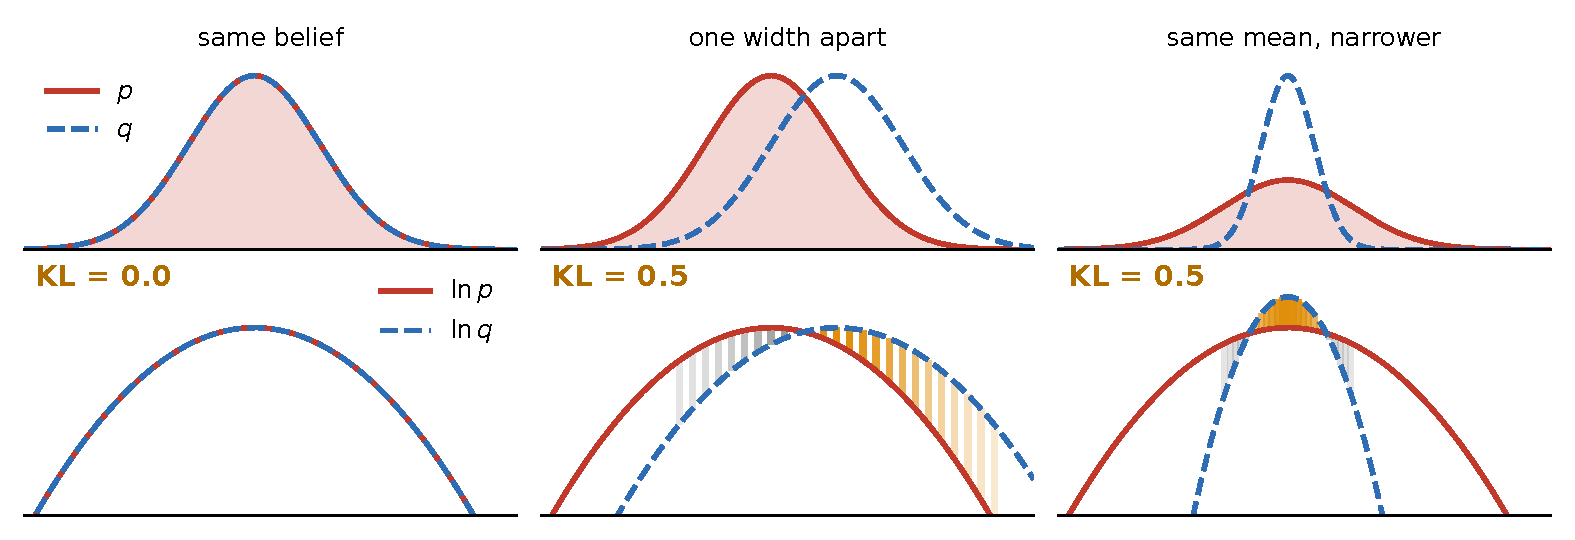
\includegraphics[width=0.82\textwidth]{d1_kl_explain.pdf}
\end{center}

\paragraph{Expectation.} The expectation of a function $f(s)$ under $q$ is the average of $f$ with every $s$ weighted by $q(s)$: $\E_q[f] = \int q(s)\,f(s)\,ds$. For $q = \N(\mu,\sigma^2)$ we need two values throughout the derivations:
\[
\E_q[s-\mu] = 0,\qquad \E_q[(s-\mu)^2] = \sigma^2 .
\]
The first holds because $q$ is symmetric around $\mu$, so the positive and negative deviations cancel. The second is the definition of the variance.

\paragraph{Entropy.} The entropy of $q$ is $-\int q\ln q\,ds = -\E_q[\ln q]$. It is large when $q$ is spread out and small when $q$ is sure. For a Gaussian, $\ln q(s) = -\tfrac12\ln(2\pi\sigma^2) - \frac{(s-\mu)^2}{2\sigma^2}$, so
\[
\E_q[\ln q] = -\tfrac12\ln(2\pi\sigma^2) - \frac{\sigma^2}{2\sigma^2} = -\tfrac12\ln(2\pi\sigma^2) - \tfrac12 = -\tfrac12\ln(2\pi e\,\sigma^2),
\]
and the entropy of $\N(\mu,\sigma^2)$ is $\tfrac12\ln(2\pi e\,\sigma^2)$. It does not depend on $\mu$.

\paragraph{From probability to $-\ln p$.} We work with $-\ln p$, a cost measured in \emph{nats} (the unit of the natural logarithm; 1 bit $= \ln 2 = 0.69$ nats). Probability $1$ costs $0$ nats, $1/2$ costs $0.69$, $1/100$ costs $4.6$. Two properties make it convenient. A product becomes a sum, $-\ln(p_1p_2) = -\ln p_1 - \ln p_2$, so the cost of independent readings adds up (Day 1's sequence: $-\ln p(o_{1:T}\given s_{1:T}) = \sum_t -\ln p(o_t\given s_t)$). A Gaussian becomes a parabola: $-\ln\N(x;0,1) = 0.92 + \tfrac12x^2$, where $0.92 = \tfrac12\ln 2\pi$. Also $\ln(a/b) = \ln a - \ln b$ is $0$ when $a = b$.

\begin{keyidea}
Expectation is an average weighted by the belief; entropy measures how spread out the belief is; $-\ln$ turns a probability into a cost in nats, and a Gaussian into a parabola. The KL of two Gaussians is a formula in their means and widths.
\end{keyidea}

\subsection{Variational Bayes and the free energy $F$}

\paragraph{The aim.} Choose, among simple beliefs $q$ (here: Gaussians), the one with the smallest $\KL{q}{p(s\given o)}$. This needs $\ln p(s\given o)$, which contains $p(o)$. The next derivation removes $p(o)$.

\paragraph{From the KL to $F$, line by line.}
\begin{align*}
\KL{q}{p(s\given o)} &= \int q\,\big[\ln q - \ln p(s\given o)\big]\,ds && (1)\\
\ln p(s\given o) &= \ln\big[p(o\given s)\,p(s)\big] - \ln p(o) && (2)\\
\KL{q}{p(s\given o)} &= \int q\,\big[\ln q - \ln\big(p(o\given s)p(s)\big) + \ln p(o)\big]\,ds && (3)\\
&= \int q\ln q\,ds - \int q\ln\big(p(o\given s)p(s)\big)\,ds + \int q\ln p(o)\,ds && (4)\\
&= \int q\,\ln\frac{q}{p(o\given s)\,p(s)}\,ds + \ln p(o)\int q\,ds && (5)\\
&= \underbrace{\int q\,\ln\frac{q}{p(o\given s)\,p(s)}\,ds}_{F[q,o]} + \ln p(o) && (6)
\end{align*}
Line (1) is the definition. (2) is Bayes' rule in logs: the log turns the division by $p(o)$ into a subtraction. (3) substitutes (2) into (1); minus a minus is a plus. (4) splits the integral in three. (5) regroups the first two integrals into one log-ratio and takes $\ln p(o)$ out of the third. (6) uses $\int q\,ds = 1$.
$\ln p(o)$ leaves the integral because it does not depend on the integration variable $s$: it is the same number at every $s$, so it is a constant factor of the third integral. What remains is the third integral $\int q\,ds\cdot\ln p(o)$, and $\int q\,ds = 1$ because $q$ is a probability density.

The first term is the \emph{variational free energy}
\[
F[q,o] = \int q(s)\,\ln\frac{q(s)}{p(o\given s)\,p(s)}\,ds = \E_q\big[\ln q(s) - \ln p(o,s)\big],\qquad p(o,s) = p(o\given s)\,p(s).
\]
It needs only the belief $q$ and the model we wrote, not $p(o)$: the robot can compute it. Moving $\ln p(o)$ to the other side gives the central identity
\[
\boxed{\,F[q,o] = \KL{q}{p(s\given o)} + \big(-\ln p(o)\big)\,}
\]
The reading $o$ fixes the second term, which is the \emph{surprise} $-\ln p(o)$. No choice of $q$ changes it. Only the KL depends on $q$, so lowering $F$ lowers the KL by the same amount. Since $\mathrm{KL} \ge 0$, we have $F \ge -\ln p(o)$: $F$ is an upper bound on the surprise, with equality when $q$ is the posterior. (In machine learning $-F$ is called the ELBO, the evidence lower bound.)

\paragraph{Check with the wall (lab Exercise 1).} The surprise is $-\ln p(o)$ with $p(o) = \N(o;\, m,\, \sigma_p^2+\sigma_o^2) = \N(2.6;\, 2.0,\, 0.29)$, which gives $p(o) = 0.398$ and $-\ln p(o) = 0.92$ nats. For three beliefs $q = \N(\mu,\sigma^2)$ the notebook gives:

\begin{center}
\begin{tabular}{@{}lccc@{}}
\toprule
belief $q$ & $F$ (nats) & KL to the posterior (nats) & $F - \mathrm{KL}$ \\
\midrule
$\N(2.0,\ 0.5^2)$ (the prior) & 6.935 & 6.014 & 0.921 \\
$\N(2.6,\ 0.1^2)$ (the reading, too sure) & 1.284 & 0.363 & 0.921 \\
$\N(2.52,\ 0.19^2)$ (the posterior) & 0.921 & 0.001 & 0.921 \\
\bottomrule
\end{tabular}
\end{center}
$F - \mathrm{KL}$ is the same for every belief: it is the surprise. $F$ never goes below $0.921$ and reaches it at the posterior.

\begin{center}
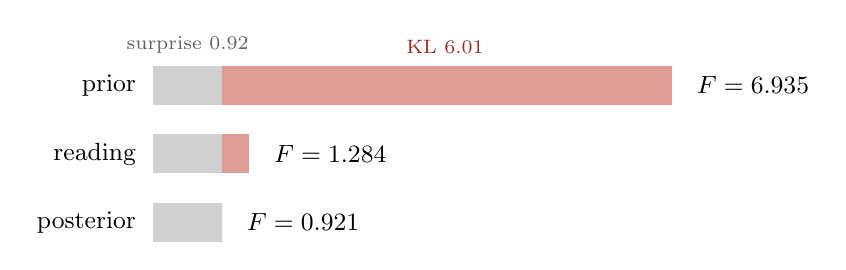
\begin{tikzpicture}[x=0.95cm, y=0.62cm]
  \foreach \y/\f/\k/\n in {0/6.935/6.014/{prior}, -1.4/1.284/0.363/{reading}, -2.8/0.921/0.0/{posterior}} {
    \fill[muted!35] (0,\y-0.4) rectangle (0.921,\y+0.4);
    \fill[accent!50] (0.921,\y-0.4) rectangle (0.921+\k,\y+0.4);
    \node[anchor=east, font=\small] at (-0.1,\y) {\n};
    \node[anchor=west, font=\small] at (\f+0.2,\y) {$F=\f$};
  }
  \node[font=\scriptsize, text=muted!80!black, anchor=south] at (0.46,0.45) {surprise 0.92};
  \node[font=\scriptsize, text=accent!80!black, anchor=south] at (3.9,0.45) {KL 6.01};
\end{tikzpicture}\\[0.2em]
{\small Each bar is $F$ in nats: grey is the surprise (the same for every belief), red is the KL.}
\end{center}

\paragraph{$F$ as the energy of two springs.} For the wall, $-\ln p(o,s) = \frac{(o-s)^2}{2\sigma_o^2} + \frac{(s-m)^2}{2\sigma_p^2} + \text{constant}$: two parabolas. Written as a physical energy, a spring stores $\tfrac12\,\text{stiffness}\times\text{stretch}^2$. So the belief's centre $\mu$ is pulled by a soft spring (stiffness $\pi_p = 4$) towards the prior $m = 2.0$ and by a stiff spring (stiffness $\pi_o = 25$) towards the reading $o = 2.6$. The total is smallest where the pulls balance, and we compute it in the next paragraphs: $\mu = (4\cdot 2.0 + 25\cdot 2.6)/29 = 2.517$. At that point the soft spring stores $\tfrac12\cdot 4\cdot 0.517^2 = 0.535$ and the stiff one $\tfrac12\cdot 25\cdot 0.083^2 = 0.086$. If the LiDAR gets worse, $\sigma_o = 0.4$ m, its stiffness drops to $1/0.4^2 = 6.25$ and the belief moves nearer the prior: $(4\cdot 2.0 + 6.25\cdot 2.6)/10.25 = 2.37$ m.

\begin{center}
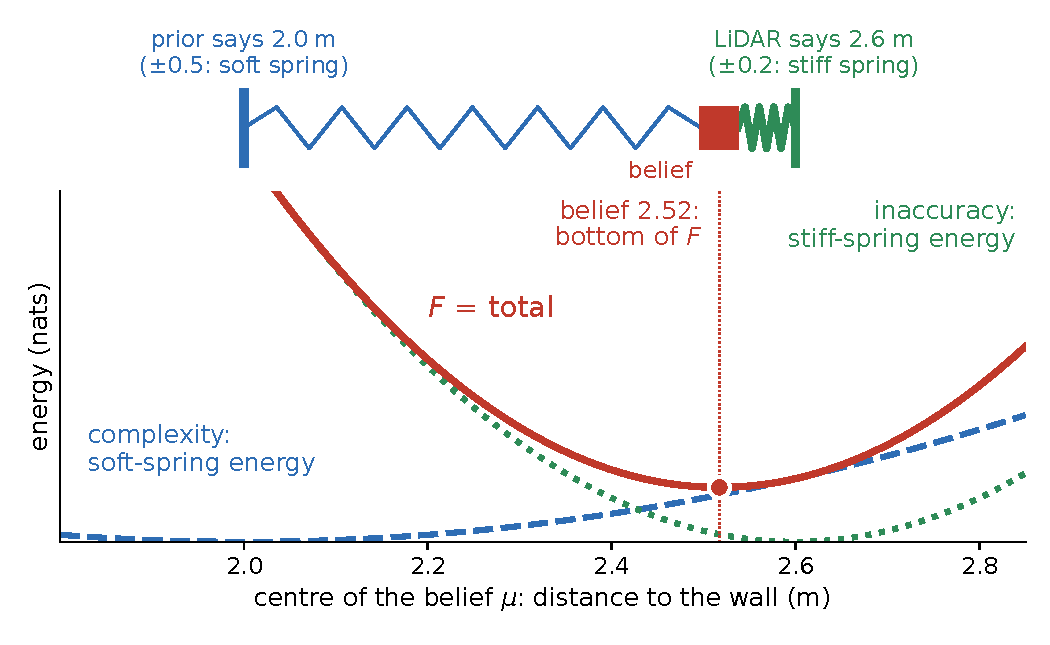
\includegraphics[width=0.62\textwidth]{d1_complexity.pdf}
\end{center}

\paragraph{$F$ = complexity $-$ accuracy.} The same $F$ can be split the other way, by writing $\ln\frac{q}{p(o\given s)p(s)} = \ln\frac{q}{p(s)} - \ln p(o\given s)$:
\[
F[q,o] = \underbrace{\KL{q(s)}{p(s)}}_{\text{complexity}} - \underbrace{\E_q\big[\ln p(o\given s)\big]}_{\text{accuracy}} .
\]
Complexity is how far the belief moved away from the prior; accuracy is how well the belief explains the reading. Leaving the prior costs complexity; explaining the reading pays accuracy. For the posterior of the wall, complexity $= 1.09$ (by the Gaussian KL formula with $\mu_1 = 2.517$, $\sigma_1 = 0.186$, $\mu_0 = 2.0$, $\sigma_0 = 0.5$) and accuracy $= 0.17$, so $F = 1.09 - 0.17 = 0.92$. Complexity corresponds to the prior's spring and the inaccuracy $-$accuracy to the reading's spring.

\paragraph{Two slopes.} Without the terms in $\sigma$ (they come in the next subsection), the springs give
\[
F(\mu, o) = \tfrac12\pi_p(\mu - m)^2 + \tfrac12\pi_o(o-\mu)^2 .
\]
$F$ depends on two things we can change, the belief's centre $\mu$ and the reading $o$, and it has a slope in each (the symbol $\partial F/\partial x$ is how fast $F$ changes when only $x$ moves):
\[
\frac{\partial F}{\partial\mu} = \pi_p(\mu - m) - \pi_o(o-\mu),\qquad \frac{\partial F}{\partial o} = \pi_o(o-\mu).
\]
Perception follows the first slope: the robot moves $\mu$. Action follows the second: the robot moves so that $o$ changes.

\begin{keyidea}
$F = \KL{q}{p(s\given o)} - \ln p(o)$ needs only $q$ and the model. Minimising $F$ over $q$ gives the belief closest to the posterior and bounds the surprise from above. Equivalent forms: surprise $+$ KL; complexity $-$ accuracy; the energy of two springs.
\end{keyidea}

\subsection{The Laplace approximation}

\paragraph{Why we need a simple $q$.} When the reading is a curved function of the state, the posterior is not Gaussian. Example from the slides: a landmark $0.8$ m to the side of a track; the range it should read at position $s$ is $h(s) = \sqrt{s^2 + 0.8^2}$, so $s = +0.6$ and $s = -0.6$ give the same range and the posterior is lopsided. We still want $q$ to be a Gaussian, and the Laplace approximation chooses it from two numbers of the curve.

\begin{center}
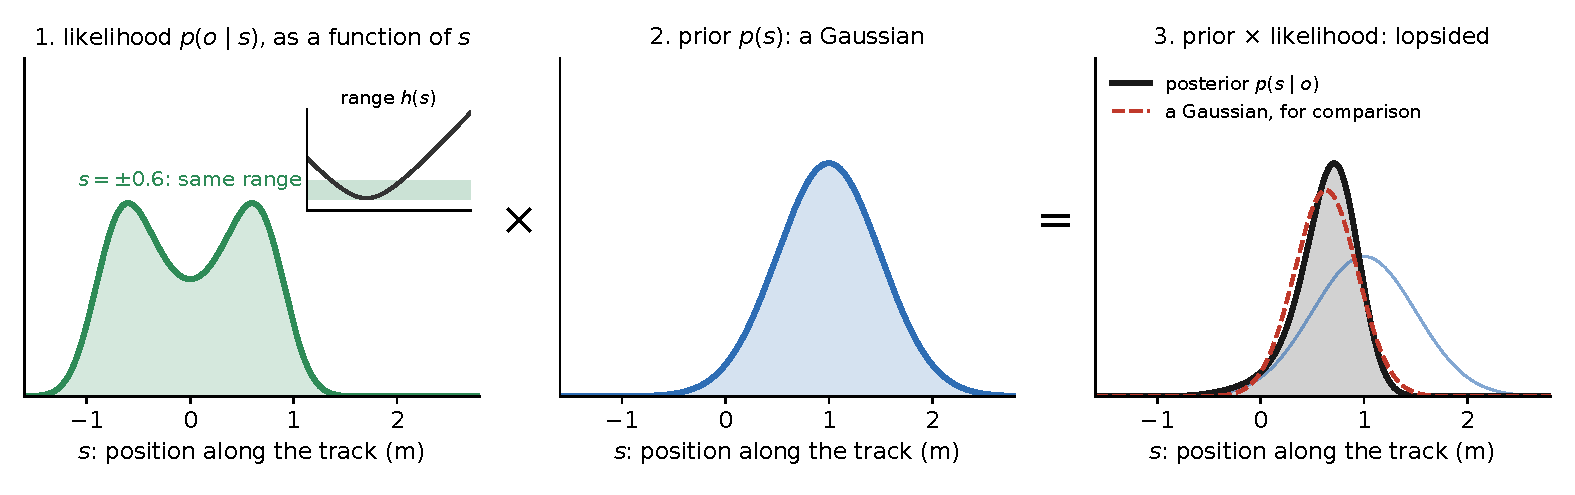
\includegraphics[width=0.85\textwidth]{d1_why_skew.pdf}
\end{center}

\paragraph{The approximation.} Take the curve we want to approximate, here $g(s) = p(o,s)$ as a function of $s$ (it is proportional to the posterior). Let $\mu$ be where $-\ln g$ is smallest (where $g$ peaks) and $\Hess$ the curvature there, $\Hess = \partial^2(-\ln g)/\partial s^2$ at $s=\mu$ (the Hessian; in one dimension, the second derivative). The Taylor expansion of $-\ln p(o,s)$ around $\mu$, up to the square, is
\[
-\ln p(o,s) \approx \underbrace{-\ln p(o,\mu)}_{\text{height at }\mu} + \underbrace{b\,(s-\mu)}_{b=0\text{ at the minimum}} + \tfrac12\Hess\,(s-\mu)^2 ,
\]
where $b = \partial(-\ln p(o,s))/\partial s$ at $\mu$ is the slope. At the minimum $b = 0$; we keep $b$ in the derivation below because it shows that the slope never matters. A parabola in $-\ln$ is a Gaussian in $p$, with mean $\mu$ and variance $1/\Hess$. So Laplace keeps two numbers: where the peak is, and how sharply $-\ln p$ bends there.

\paragraph{$F$ under Laplace, line by line.} Let the belief be $q = \N(\mu,\sigma^2)$, with $\mu$ its mean and $\sigma$ its width (both to be chosen). Start from $F = \E_q[\ln q - \ln p(o,s)]$ and split the log:
\begin{align*}
F &= \underbrace{\E_q[\ln q(s)]}_{\text{minus the entropy of }q} + \E_q\big[-\ln p(o,s)\big]\\
&\approx -\tfrac12\ln(2\pi e\sigma^2) + \E_q\big[-\ln p(o,\mu) + b(s-\mu) + \tfrac12\Hess(s-\mu)^2\big] && \text{\small entropy; parabola}\\
&= -\tfrac12\ln(2\pi e\,\sigma^2) - \ln p(o,\mu) + b\,\underbrace{\E_q[s-\mu]}_{=0} + \tfrac12\Hess\,\underbrace{\E_q[(s-\mu)^2]}_{=\sigma^2} && \text{\small average term by term}\\
&= -\ln p(o,\mu) + \tfrac12\Hess\,\sigma^2 - \tfrac12\ln(2\pi e\,\sigma^2) .
\end{align*}
In the third line, $-\ln p(o,\mu)$ has no $s$ so its average is itself; the slope term averages to zero because $\E_q[s-\mu] = 0$, whatever the value of $b$; and $\E_q[(s-\mu)^2] = \sigma^2$. The result has three terms and no integral:
\[
\boxed{\,\Fl(\mu,\sigma) = \underbrace{-\ln\big[p(o\given\mu)\,p(\mu)\big]}_{\text{misfit of the mean}} + \underbrace{\tfrac12\Hess\,\sigma^2}_{\text{cost of spreading}} - \underbrace{\tfrac12\ln(2\pi e\,\sigma^2)}_{\text{entropy of }q\text{: reward for spreading}}\,}
\]
For the wall (a linear sensor and Gaussian factors), the parabola is exact, so this formula is not an approximation there: $F(\mu,\sigma) = \tfrac12\ln(2\pi\sigma_o^2) + \tfrac12\ln(2\pi\sigma_p^2) + \frac{(o-\mu)^2 + \sigma^2}{2\sigma_o^2} + \frac{(\mu-m)^2+\sigma^2}{2\sigma_p^2} - \tfrac12\ln(2\pi e\sigma^2)$. Collecting the terms in $\sigma^2$ gives $\tfrac12(\pi_o+\pi_p)\sigma^2$, so $\Hess = 29$.

\paragraph{Why $\sigma^2 = 1/\Hess$.} Only two terms of $\Fl$ contain $\sigma$. The cost $\tfrac12\Hess\sigma^2$ grows with $\sigma$; the entropy reward $-\tfrac12\ln(2\pi e\sigma^2)$ falls with $\sigma$. The sum has a minimum between them. Differentiate with respect to $\sigma$, using $\tfrac{d}{d\sigma}\tfrac12\Hess\sigma^2 = \Hess\sigma$ and $\tfrac{d}{d\sigma}\big[-\tfrac12(\ln 2\pi e + 2\ln\sigma)\big] = -\tfrac1\sigma$:
\[
\frac{\partial F}{\partial\sigma} = \Hess\,\sigma - \frac{1}{\sigma} = 0 \;\Longrightarrow\; \sigma^2 = \frac{1}{\Hess}.
\]
It is a minimum because $\partial^2F/\partial\sigma^2 = \Hess + 1/\sigma^2 > 0$. A sharp bowl (large $\Hess$) gives a small $\sigma$: a sure belief. For the mean, $\Hess$ is held fixed, so only $-\ln p(o,\mu)$ depends on $\mu$, and the best $\mu$ is the minimum of $-\ln p(o,s)$. For the wall, $\Hess = \pi_p + \pi_o = 4 + 25 = 29$, so $\sigma = 1/\sqrt{29} = 0.186$ m: precisions add. The slides' figure shows the same balance for the landmark at two readings ($\Hess = 24$, $\sigma = 0.20$ m; $\Hess = 16$, $\sigma = 0.25$ m).

\begin{center}
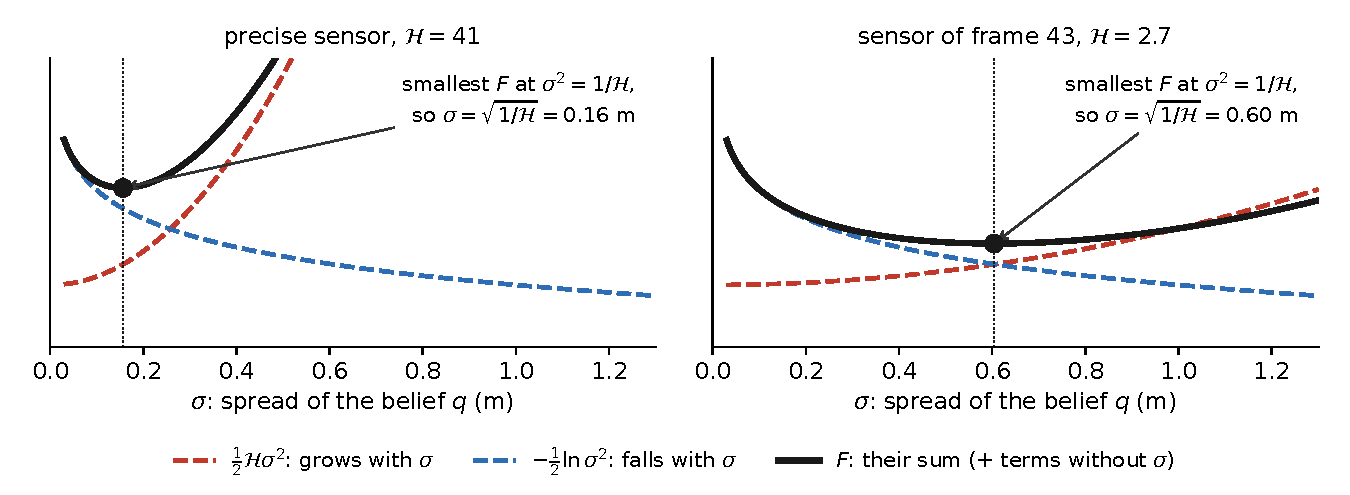
\includegraphics[width=0.72\textwidth]{d1_sigma_balance.pdf}
\end{center}

\paragraph{The value of $F$ at the minimum.} Put $\sigma^2 = 1/\Hess$ back: $\tfrac12\Hess\sigma^2 = \tfrac12$ and $-\tfrac12\ln(2\pi e/\Hess) = -\tfrac12\ln 2\pi - \tfrac12 + \tfrac12\ln\Hess$, so
\[
F_{\min} = -\ln p(o,\mu) + \tfrac12\ln\frac{\Hess}{2\pi}.
\]
This is the Laplace estimate of the surprise $-\ln p(o)$. For the wall: $-\ln p(o,\mu) = 0.156$ and $\tfrac12\ln(29/2\pi) = 0.765$, which add to $0.921$, the exact surprise. In lab Exercise 2 you find this numerically.

\begin{keyidea}
With $q = \N(\mu,\sigma^2)$ and a parabola for $-\ln p(o,s)$, $F$ is a formula in $\mu$ and $\sigma$: a misfit, a cost of spreading and an entropy. Its minimum is at the bottom of the parabola for $\mu$, and at $\sigma^2 = 1/\Hess$ for the spread.
\end{keyidea}

\subsection{Minimising $F$: perception and action}

\paragraph{Gradient steps.} To lower $F$ by a quantity $x$ the robot repeats $x \leftarrow x - \eta\,\partial F/\partial x$, where $\eta$ is a step size. This moves $x$ against the slope; the steps shrink as the slope flattens near the minimum. Perception does it with $x = \mu$ (move the belief); action does it with $x = a$ (move the robot), where $a$ is the command sent to the wheels (here, how far the robot drives).

\paragraph{Perception.} With a sensor $h$ that maps the state to the reading the robot expects, the model is $p(o\given\mu)\propto e^{-\frac12\pi_o(o-h(\mu))^2}$ and $p(\mu)\propto e^{-\frac12\pi_p(\mu-m)^2}$ (precisions $\pi_o = 1/\sigma_o^2$, $\pi_p = 1/\sigma_p^2$). Take the logs, drop the terms in $\sigma$ and the constants:
\[
F(\mu,o) = \tfrac12\pi_o\,\big(o - h(\mu)\big)^2 + \tfrac12\pi_p(\mu-m)^2 .
\]
By the chain rule, $\frac{d}{d\mu}\tfrac12\pi_o(o-h(\mu))^2 = \pi_o\,(o-h(\mu))\cdot(-h'(\mu))$, hence
\[
\frac{\partial F}{\partial\mu} = -\pi_o\,\underbrace{\big(o-h(\mu)\big)}_{\text{prediction error}}\,h'(\mu) + \pi_p(\mu - m),\qquad \mu\leftarrow\mu - \eta\,\frac{\partial F}{\partial\mu}.
\]
$h'$ is the slope of $h$. The prediction error is the reading minus what the belief predicts. The belief moves by the prediction error weighted by the reading's precision, against the pull of the prior. For the wall, $h(\mu) = \mu$ and $h' = 1$.

\paragraph{The Kalman update is the minimum of $F$.} For $h(s) = s$ set $\partial F/\partial\mu = 0$:
\[
\pi_p(\mu - m) - \pi_o(o-\mu) = 0 \;\Longrightarrow\; \mu = \frac{\pi_p\,m + \pi_o\,o}{\pi_p + \pi_o},\qquad \frac{1}{\sigma^2} = \Hess = \pi_p + \pi_o,
\]
the second from $\partial^2F/\partial\mu^2 = \pi_p+\pi_o$. This is Kalman's update, in Day 1's names $m = \mu_-$, $\pi_p = 1/\sigma_-^2$, $\pi_o = 1/\sigma_v^2$: the new mean is the average of prior and reading weighted by precision, and the precisions add. Wall: $\mu = (4\cdot2.0 + 25\cdot2.6)/29 = 2.517$ m, $\sigma = 0.186$ m. Kalman's formula jumps to the minimum in one step; gradient descent walks there. For a nonlinear $h$ the gradient steps get there too (the lab, section 2, does the linear case step by step: from $\mu = 2.0$ the slope is $-25\cdot0.6 = -15$, so with $\eta = 0.01$ the first step goes to $2.15$, the next to $2.2565$).

\paragraph{Action.} Now the reading depends on what the robot does: $o = o(a)$. The same $F$ gives, by the chain rule,
\[
\frac{\partial F}{\partial a} = \frac{\partial F}{\partial o}\,\frac{\partial o}{\partial a} = \pi_o\,\big(o - h(\mu)\big)\,\frac{\partial o}{\partial a},\qquad a\leftarrow a - \eta\,\frac{\partial F}{\partial a}.
\]
$\partial F/\partial o = \pi_o(o - h(\mu))$ is the second slope of Section~1.3; $\partial o/\partial a$ is how the reading changes with the command, and it is the part that needs a model of the robot's body and sensor. The prediction error is the same one that drives perception, but now the robot reduces it by changing $o$ instead of $\mu$.

\paragraph{Action as a proportional controller, and the sign.} Take $h(\mu)=\mu$. Then $a\leftarrow a - \eta\pi_o\,\frac{\partial o}{\partial a}\,(o - \mu)$, so the change in $a$ in one step is
\[
\Delta a = -\eta\,\pi_o\,\frac{\partial o}{\partial a}\,(o-\mu) = \eta\,\pi_o\,\frac{\partial o}{\partial a}\,(\mu - o).
\]
A proportional controller computes $\Delta a = K_P\,(\text{set point} - \text{measurement})$. Here the set point is the robot's own prediction $\mu$, the measurement is the reading $o$, and the gain is $K_P = \eta\,\pi_o\,\partial o/\partial a$: a more precise reading (larger $\pi_o$) gives a larger gain. If the prior holds what the robot wants, the prediction becomes a desire and action makes it come true (Day 4).

The sign lives in $\partial o/\partial a$. Let $a$ be the distance driven towards the wall. Driving towards the wall shortens the range, so $\partial o/\partial a = -1$. Then $\Delta a = \eta\pi_o\,(o-\mu)$. If the reading is longer than the prediction ($o>\mu$) then $\Delta a>0$: the robot drives forward, the range shrinks, and the error $o-\mu$ goes to zero. If the reading is shorter ($o<\mu$) then $\Delta a<0$ and the robot backs off. With the opposite sign convention for $a$ (distance backed away from the wall) $\partial o/\partial a = +1$ and the update has the opposite sign, and it is still the same behaviour: the signs of the controller and of the plant multiply.

\begin{keyidea}
The same prediction error $o - h(\mu)$ drives both. Perception changes $\mu$ by $\pi_o\,(o-h(\mu))\,h'(\mu)$ against the prior's pull; action changes $a$ so that the reading approaches the prediction, which is a proportional controller whose gain is $\eta\pi_o\,\partial o/\partial a$.
\end{keyidea}

\subsection{Planning into the future: the expected free energy $G$}

\paragraph{Imagined readings.} Perception uses readings from before ``now''. To choose an action the robot needs the readings it would get after it, which do not exist yet. It runs its own model forward, in the order of the slide's timeline:
\begin{center}
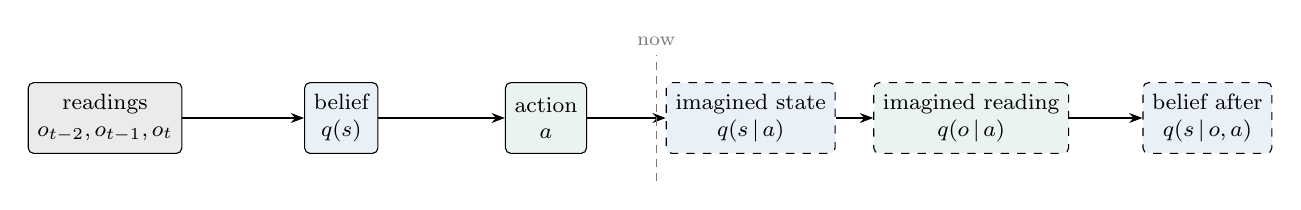
\begin{tikzpicture}[x=1cm, y=1cm, bx/.style={draw, rounded corners=2pt, minimum height=0.9cm, align=center, font=\footnotesize}]
  \node[bx, fill=muted!15] (past) at (0,0) {readings\\$o_{t-2},o_{t-1},o_t$};
  \node[bx, fill=cool!10] (b0) at (3.0,0) {belief\\$q(s)$};
  \node[bx, fill=good!10] (a) at (5.6,0) {action\\$a$};
  \node[bx, fill=cool!10, dashed] (s) at (8.2,0) {imagined state\\$q(s\given a)$};
  \node[bx, fill=good!10, dashed] (o) at (11.0,0) {imagined reading\\$q(o\given a)$};
  \node[bx, fill=cool!10, dashed] (b1) at (14.0,0) {belief after\\$q(s\given o,a)$};
  \draw[-{Stealth}] (past)--(b0); \draw[-{Stealth}] (b0)--(a); \draw[-{Stealth}] (a)--(s); \draw[-{Stealth}] (s)--(o); \draw[-{Stealth}] (o)--(b1);
  \draw[densely dashed, muted] (7.0,-0.8) -- (7.0,0.8) node[above, font=\scriptsize] {now};
\end{tikzpicture}
\end{center}
\vspace{-0.5em}
The motion model gives the imagined state $q(s\given a)$, the sensor model $p(o\given s)$ gives an imagined reading, and a Day 1 update (Kalman) gives the belief after reading it, $q(s\given o,a)$. Nothing has happened: every box after ``now'' is computed with the model. (The picture is scaled to fit; read it left to right.)

\paragraph{Two reasons to act.} An action is good if it \emph{teaches} something (the belief would sharpen) or if it brings the readings close to a goal. The goal is a distribution over readings the robot prefers, $\tilde p(o) = \N(o;\, o^*,\sigma_*^2)$: $o^*$ is the reading it wants and $\sigma_*$ says how strict the goal is. Then $-\ln\tilde p(o) = \frac{(o-o^*)^2}{2\sigma_*^2} + \text{constant}$, the squared distance to the goal in units of the goal's width.

\paragraph{How the robot computes $G$: imagine, update, score, average.} For one action $a$ the robot repeats:
\begin{enumerate}[nosep, label=\textbf{\arabic*.}]
\item \textbf{imagine the state}: draw $s$ from $q(s\given a)$ (motion model);
\item \textbf{imagine a reading}: draw $o$ from $p(o\given s)$ (sensor model);
\item \textbf{update as if $o$ were real}: Kalman gives $q(s\given o,a)$;
\item \textbf{score}: how much narrower the belief became, and how far $o$ is from the goal.
\end{enumerate}
It averages the score over many imagined readings; this average is $G(a)$, and the robot picks the action with the lowest $G$. For a Gaussian belief the learning part has a closed form, derived below: $\tfrac12\ln(\sigma^2_{\text{before}}/\sigma^2_{\text{after}})$, with the minus sign in $G$, plus $(o - o^*)^2/(2\sigma_*^2)$ for the goal.

\paragraph{Where $G$ comes from (lab Exercise 3).} $F$ is an average over the belief for \emph{one} reading we have. $G$ has the same form, but averages over readings the robot only imagines, with the goal as prior over readings:
\[
F = \E_{q(s)}\big[\ln q(s) - \ln p(o,s)\big],\qquad
G(a) = \E_{q(o,s\given a)}\big[\ln q(s\given a) - \ln\tilde p(o,s)\big] .
\]
Here $q(s\given a)$ is the belief after action $a$ and before any reading; $q(o,s\given a) = q(s\given a)\,p(o\given s)$ is the joint distribution of imagined states and readings; $\tilde p(o,s)$ is the model with the goal as the prior over readings. We split $G$ in three steps.

\begin{align*}
G(a) &= \E\big[\ln q(s\given a) - \ln\tilde p(o,s)\big] && \text{every }\E\text{ is over }q(o,s\given a)\\
&\approx \E\big[\ln q(s\given a) - \ln q(s\given o,a) - \ln\tilde p(o)\big] && \tilde p(o,s)\approx q(s\given o,a)\,\tilde p(o)\\
&= -\E\big[\ln q(s\given o,a) - \ln q(s\given a)\big] - \E\big[\ln\tilde p(o)\big] && \text{regroup the first two logs}
\end{align*}
The approximation in the second line says: the joint $\tilde p(o,s)$ is the belief about $s$ after reading $o$, times the preference for $o$ (the product rule $p(o,s) = p(s\given o)p(o)$, with the belief after reading in place of the exact conditional). The third line only regroups: $\ln q(s\given a) - \ln q(s\given o,a) = -[\ln q(s\given o,a) - \ln q(s\given a)]$. Now average the first bracket. Because $q(o,s\given a) = q(o\given a)\,q(s\given o,a)$, an average over the pair is an average over $o$ of an average over $s$ given $o$, and the inner average of $\ln q(s\given o,a) - \ln q(s\given a)$ under $q(s\given o,a)$ is by definition a KL:
\[
\boxed{\,G(a) = \underbrace{-\,\E_{q(o\given a)}\Big[\KL{q(s\given o,a)}{q(s\given a)}\Big]}_{\text{what the action would teach}}\;\underbrace{-\;\E_{q(o\given a)}\big[\ln\tilde p(o)\big]}_{\text{how far it leaves the goal}}\,}
\]
The first term is minus the average KL between the belief after and before the reading: the more the belief would change, the lower $G$. The second is the goal term. Both are in nats, so they add directly.

\paragraph{Why the learning term has a minus, and why that is a choice.} The minus comes from $\ln q(s\given a)$ having a plus sign in $G$ while $\ln q(s\given o,a)$ has a minus: $G$ is written with the belief \emph{before} the reading inside the expectation. It is not forced by the mathematics. Other definitions of the expected free energy exist, and Millidge, Tschantz and Buckley (\emph{Whence the expected free energy?}, Neural Computation, 2021) discuss how they differ. We use this one: a lower $G$ means more learned.

\paragraph{The learning term for a Gaussian.} Let the belief before the reading be $\N(\mu_b,\sigma_b^2)$ and the sensor noise $\sigma_o$. The Kalman update after reading $o$ gives $\sigma_a^2 = (1-k)\sigma_b^2$ and $\mu_a = \mu_b + k\,(o-\mu_b)$ with $k = \sigma_b^2/(\sigma_b^2+\sigma_o^2)$. The KL of one imagined reading is
\[
\KL{\N(\mu_a,\sigma_a^2)}{\N(\mu_b,\sigma_b^2)} = \tfrac12\ln\frac{\sigma_b^2}{\sigma_a^2} + \frac{\sigma_a^2 + (\mu_a-\mu_b)^2}{2\sigma_b^2} - \tfrac12 .
\]
The imagined reading has $\E[(o-\mu_b)^2] = \sigma_b^2 + \sigma_o^2$, so $\E[(\mu_a-\mu_b)^2] = k^2(\sigma_b^2+\sigma_o^2) = k\,\sigma_b^2$. The average of the last two terms is $\frac{(1-k)\sigma_b^2 + k\sigma_b^2}{2\sigma_b^2} - \tfrac12 = 0$, and what is left is
\[
\E_o\big[\mathrm{KL}\big] = \tfrac12\ln\frac{\sigma_b^2}{\sigma_a^2} = \tfrac12\ln\Big(1 + \frac{\sigma_b^2}{\sigma_o^2}\Big),
\]
using $1/\sigma_a^2 = 1/\sigma_b^2 + 1/\sigma_o^2$. A single imagined reading has an extra term for how far the mean moved; it cancels on average. With $\sigma_b = 0.5$ (the wall's prior): sensor $\sigma_o = 0.1$ gives $\tfrac12\ln 26 = 1.629$ nats; $\sigma_o = 1.0$ gives $\tfrac12\ln 1.25 = 0.112$ nats. The good sensor teaches fourteen times more.

\begin{keyidea}
$G(a)$ is $F$ averaged over the readings an action would bring, with the goal as the prior over readings. It splits into what the action would teach (minus the expected KL from the belief before to the belief after reading) and how far it leaves the readings from the goal. The robot computes it by imagining, updating, scoring and averaging; it picks the lowest $G$.
\end{keyidea}

%=====================================================================================
\section{Backup slides}
%=====================================================================================

\begin{backupbox}{Backup 1: is the belief's spread right? Scan 400 times from the same place}
$d$ is the robot--wall distance estimated from one scan, and $\sigma_d$, with $\sigma_d^2 = 1/\Hess$, is the spread of the belief. It is a \emph{claim}: how far $d$ would typically move if you scanned again. To test it, fit 400 scans taken from the same pose and compare the scatter of the 400 estimates with the claim. The slide shows the histogram of $d$ minus its mean (millimetres), with two predictions drawn on it.

\begin{center}
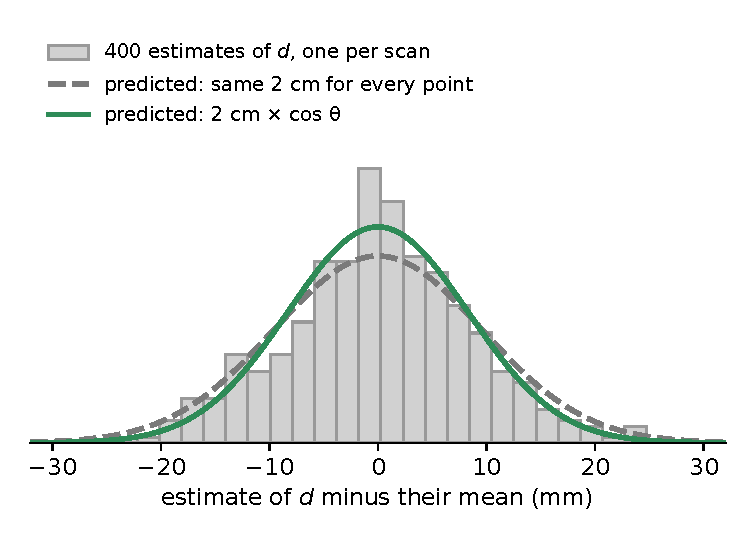
\includegraphics[width=0.48\textwidth]{d2_spread_check.pdf}
\end{center}

The first prediction (grey) is the likelihood we wrote first: every point has the same noise, 2 cm. It is a few per cent too wide. The reason: the LiDAR error $\epsilon$ is along the \emph{beam}, with direction $u$, but $d$ is measured along the wall's \emph{normal} $n$. A range error $\epsilon$ moves the point by $\epsilon\,(u^\top n)$ off the wall, so the point's standard deviation is $2\text{ cm}\times|u^\top n| = 2\text{ cm}\times\cos\theta$, where $\theta$ is the angle between the beam and the normal ($\theta = 0$ is head-on). Only the error across the wall moves $d$; the error along the wall slides the point without changing the fit. With this per-point $\sigma_i$ (green) the prediction matches the scatter.

\textbf{Lesson.} A belief's spread is only as right as the noise model we wrote. The Laplace covariance is exactly as good as the likelihood.
\end{backupbox}

\begin{backupbox}{Backup 2: $F$ also compares models: an extra parameter stays only if it lowers $F$}
We write two models of the same wall. \emph{Fixed}: the wall's normal angle is $\alpha = 90^\circ$, known; the model estimates only $d$. \emph{Free}: prior $\alpha\sim\N(90^\circ, s^2)$ and it estimates $\alpha$ and $d$ ($s$ is the width of the prior on the angle; the slide uses $s = 5^\circ$). For a wall of unit normal $n(\alpha) = (\cos\alpha, \sin\alpha)$ the residual of point $i$ at $(x_i,y_i)$ is $r_i = \cos\alpha\,x_i + \sin\alpha\,y_i - d$. Both models are Laplace beliefs, so each has an $F_{\min}$ (Section~1.4, ``The value of $F$ at the minimum'', now with a $2\times2$ curvature matrix), an estimate of $-\ln p(o\given\text{model})$. The difference is a log Bayes factor in nats; lower $F$ wins:
\[
F_{\text{free}} - F_{\text{fixed}} = \underbrace{\Delta(\text{misfit})}_{-\ln p(o\given\mu):\ \text{how badly the fit explains the scan}} + \underbrace{\Delta(\text{complexity})}_{\text{how far the belief moved from its prior}} .
\]
The free model can only fit better, so $\Delta$misfit $\le 0$; it also has one more parameter to move away from its prior, so $\Delta$complexity $>0$.

\textbf{Wall at $90^\circ$:} the fit gains almost nothing (the extra angle stays at $90^\circ$), but the belief about the angle still has to be squeezed from the prior width $s$ to the much narrower posterior width, and complexity charges for it: roughly $\ln(s/\sigma_\alpha)$ nats, with $\sigma_\alpha$ the posterior width. In the notebook, $F_{\text{free}} - F_{\text{Manhattan}}$ grows from $0.22$ nats at $s = 0.1^\circ$ to $3.6$ nats at $s = 5^\circ$ and $5.4$ at $s = 30^\circ$: the fixed model wins.

\textbf{Wall tilted by $1.5^\circ$:} a tilt of $1.5^\circ$ over the $3.9$ m span of the scan moves the end points by $\pm 0.05$ m from the fixed model's line, far more than the $2$ cm noise, so the misfit of the fixed model is large. The accuracy term outweighs the complexity: in the notebook $F_{\text{free}} - F_{\text{Manhattan}} = -87.4$ nats at $s = 5^\circ$, and the free model wins.

\textbf{Lesson.} Nobody wrote ``if the angle error exceeds $k$ degrees, abandon the Manhattan model''. The decision falls out of comparing two free energies: an extra parameter stays only if its better fit outweighs its complexity.
\end{backupbox}

%=====================================================================================
\section{Lab guide}
%=====================================================================================

The notebook is \texttt{labs/day2.ipynb}. Everything you write goes between the \texttt{BEGIN SOLUTION} and \texttt{END SOLUTION} markers; the rest is given. The numbers below are what a correct solution prints (the Monte Carlo ones change slightly with the random seed's stream). See the cheat sheet for numpy (arrays, \texttt{sum}, \texttt{mean}, broadcasting, \texttt{argmin}) and for the Gaussian formulas.

\subsection*{Section 1: three derivations by hand (in class: the checks; the derivations of Exercises 1 and 3 at home)}
Pen and paper first, then the numerical check. The setup cell defines the wall: \texttt{m, sigma\_p = 2.0, 0.5}; \texttt{o, sigma\_o = 2.6, 0.2}; a grid \texttt{s} with step \texttt{ds}; the joint \texttt{joint = p(o|s) p(s)} on the grid; \texttt{p\_o = joint.sum()*ds}; and \texttt{posterior = joint/p\_o}. It prints $p(o) = 0.398$ and the surprise $0.921$ nats.

\begin{labhelp}{Exercise 1: the free energy}
\textbf{Goal.} Show $\KL{q}{p(s\given o)} = F + \ln p(o)$, say why $F\ge -\ln p(o)$, and check numerically.\\
\textbf{Slide.} Kullback--Leibler divergence; Bayes in logs; ``Substitute: $\ln p(o)$ leaves the integral''. Full derivation: Section~1.3 of this handout.\\
\textbf{Steps.} (1) Write the KL as $\int q\,[\ln q - \ln p(s\given o)]$. (2) Replace $\ln p(s\given o)$ by Bayes in logs. (3) Split into three integrals. (4) Pull $\ln p(o)$ out, because it has no $s$. (5) Use $\int q = 1$. (6) The remaining integral is $F$. (7) KL $\ge0$ gives $F\ge-\ln p(o)$; equality when $q$ is the posterior.\\
\textbf{Code.} \texttt{free\_energy(mu, sd)}: on the grid, $F\approx\sum_s q\,(\ln q - \ln \texttt{joint})\,ds$. \texttt{kl\_to\_posterior}: the same with \texttt{posterior} instead of \texttt{joint}. Arrays have the shape of \texttt{s}, $(6001,)$.\\
\textbf{Check.} The printed lines should read\\
\texttt{N(2.0,0.5): F = 6.935 KL = 6.014 F-KL = 0.921};\ \ \texttt{N(2.6,0.1): 1.284, 0.363, 0.921};\ \ \texttt{N(2.52,0.19): 0.921, 0.001, 0.921}.\\
\textbf{Common mistakes.} Forgetting to multiply by \texttt{ds} (every number is then $1/0.001$ too large). Taking $\ln 0$: where $q$ underflows to $0$ the product $q\ln q$ is $0$, so keep only the points with \texttt{q > 1e-300} (the given code does this with a boolean mask; apply the mask to \texttt{q}, to \texttt{joint} and to \texttt{posterior}). Using \texttt{np.log(q/joint)} without the mask gives \texttt{nan}.
\end{labhelp}

\begin{labhelp}{Exercise 2: $F$ under Laplace, and $\sigma^2=1/\Hess$}
\textbf{Goal.} Show $F(\mu,\sigma)\approx-\ln p(o,\mu)+\tfrac12\Hess\sigma^2-\tfrac12\ln(2\pi e\sigma^2)$; minimise over $\sigma$; compute $\Hess$ for the wall.\\
\textbf{Slide.} The Laplace approximation; ``Why $\sigma^2=1/\Hess$''. Full derivation: Section~1.4.\\
\textbf{Steps.} (1) $F = \E_q[\ln q] + \E_q[-\ln p(o,s)]$. (2) Entropy of a Gaussian for the first term. (3) Insert the parabola with slope $b$ and curvature $\Hess$. (4) Average each term: $\E_q[s-\mu]=0$, $\E_q[(s-\mu)^2]=\sigma^2$. (5) Differentiate in $\sigma$: $\Hess\sigma-1/\sigma=0$. (6) For the wall, $-\ln p(o,s)=\frac{(o-s)^2}{2\sigma_o^2}+\frac{(s-m)^2}{2\sigma_p^2}+\text{const}$, so $\partial^2/\partial s^2 = 1/\sigma_o^2 + 1/\sigma_p^2$.\\
\textbf{Code.} \texttt{Fgrid[i,j] = free\_energy(mus[i], sds[j])} for the grids \texttt{mus} (81 values from 2.3 to 2.7) and \texttt{sds} (51 values from 0.10 to 0.35); then \texttt{np.unravel\_index(Fgrid.argmin(), Fgrid.shape)} gives $(i,j)$ of the minimum. \texttt{Fgrid} has shape $(81,51)$.\\
\textbf{Check.} $\Hess=29$, $1/\sqrt{\Hess}=0.186$. Output: \texttt{minimum at mu = 2.515, sigma = 0.185} (the grid steps are 0.005, so these differ from $2.517$ and $0.186$ in the third digit) and \texttt{F at the minimum = 0.921 = surprise}. The answer to ``why'': the sensor is linear and both factors are Gaussian, so the exact posterior is Gaussian and the best $q$ equals it, the KL is $0$, and $F$ touches the surprise.\\
\textbf{Common mistakes.} Writing $\sigma$ where $\sigma^2$ belongs in $\tfrac12\Hess\sigma^2$. Forgetting that $\partial/\partial\sigma$ of $-\tfrac12\ln\sigma^2$ is $-1/\sigma$, not $-1/\sigma^2$. Looking for the minimum at the edge of the grid: if it is there, the grid does not contain the minimum.
\end{labhelp}

\begin{labhelp}{Exercise 3: splitting the expected free energy}
\textbf{Goal.} Show $G(a) = -\E[\KL{q(s\given o,a)}{q(s\given a)}] - \E[\ln\tilde p(o)]$, then compute the learning term by imagination.\\
\textbf{Slide.} ``How the robot computes $G$: imagine, update, score, average''; ``To choose an action, score the readings it would bring''. Full derivation: Section~1.5.\\
\textbf{Steps (derivation).} (1) Insert $\tilde p(o,s)\approx q(s\given o,a)\tilde p(o)$. (2) The log of a product is a sum. (3) Regroup the two beliefs into $-[\ln q(s\given o,a)-\ln q(s\given a)]$. (4) Write the average over $q(o,s\given a)$ as an average over $o$ of an average over $s$ given $o$. (5) The inner average is a KL. (6) Say where the minus sign comes from (a choice; Millidge et al., 2021).\\
\textbf{Code: \texttt{learning\_term(mu\_b, sd\_b, sigma\_obs, n)}, one numpy line per step, all arrays of shape \texttt{(n,)}.} (1) \texttt{s\_img = rng.normal(mu\_b, sd\_b, n)}; (2) \texttt{o\_img = rng.normal(s\_img, sigma\_obs)}; (3) the gain \texttt{k = sd\_b**2/(sd\_b**2 + sigma\_obs**2)}, then \texttt{mu\_a = mu\_b + k*(o\_img - mu\_b)} and \texttt{sd\_a = np.sqrt((1-k)*sd\_b**2)}; (4) \texttt{kl\_gauss(mu\_a, sd\_a, mu\_b, sd\_b).mean()}. $k$ is a single number; \texttt{mu\_a} has shape \texttt{(n,)}, \texttt{sd\_a} is a number.\\
\textbf{Check.} Sensor $0.1$: imagined average about $1.626$, formula $1.629$ nats; sensor $1.0$: about $0.111$, formula $0.112$. The two agree to a few thousandths. The derivation is in Section~1.5, ``The learning term for a Gaussian''.\\
\textbf{Common mistakes.} Putting a standard deviation where a variance belongs in $k$. Swapping the two beliefs in \texttt{kl\_gauss} (it is $\KL{\text{after}}{\text{before}}$, not the reverse). Averaging before taking the KL (the KL of the average belief is not the average KL). Drawing \texttt{o\_img} from the sensor noise only, without \texttt{s\_img}.
\end{labhelp}

\subsection*{Section 2: perception, one step at a time (10 min)}

\begin{labhelp}{Exercise 4: gradient descent on the belief}
\textbf{Goal.} Walk $\mu$ to the minimum of $F$ with gradient steps, and see why too large a step diverges.\\
\textbf{Slide.} ``Perception: the belief follows the precision-weighted prediction error''; ``The Kalman update is free-energy minimisation''. Section~1.5.\\
\textbf{Steps.} $F(\mu)=\tfrac12\pi_o(o-\mu)^2+\tfrac12\pi_p(\mu-m)^2$ with $\pi_o=25$, $\pi_p=4$. Start at $\mu=m$. Repeat 100 times: compute the slope $-\pi_o(o-\mu)+\pi_p(\mu-m)$, then \texttt{mu -= eta * slope}, then append \texttt{mu} to the path.\\
\textbf{Code.} The loop inside \texttt{descend(eta, steps=100)} is three lines. \texttt{path} has $101$ entries.\\
\textbf{Check.} First slope at $\mu=2.0$ is $-15$, so with $\eta=0.01$ the path goes $2.0\to2.15\to2.2565$. After $100$ steps: $\eta=0.01$: $2.517$; $\eta=0.06$: $2.517$ (it overshoots and oscillates, but settles); $\eta=0.08$: $-5.9\times10^{11}$ (diverges). Kalman: $2.5172$; the minimum from Exercise 2: $2.515$ on the grid.\\
\textbf{Why $\eta=0.08$ diverges.} Since $F$ is a parabola, the slope is $\Hess\,(\mu-\mu^*)$ with $\Hess=\pi_p+\pi_o=29$ and $\mu^*=2.517$ the minimum. One step gives $\mu_{k+1}-\mu^* = (1-\eta\Hess)(\mu_k-\mu^*)$: each step multiplies the error by $1-\eta\Hess$. For $\eta=0.01$ the factor is $0.71$ (the error shrinks smoothly); for $\eta=0.06$ it is $-0.74$ (the sign alternates, the size shrinks); for $\eta=0.08$ it is $-1.32$, larger than $1$ in size, so after $100$ steps the error is $1.32^{100}\approx10^{12}$ times larger. The step must satisfy $|1-\eta\Hess|<1$, i.e.\ $\eta<2/\Hess=2/29\approx0.069$: the sharper the minimum, the smaller the step. Kalman needs no step size because it solves $\partial F/\partial\mu=0$ directly.\\
\textbf{Common mistakes.} A wrong sign (\texttt{mu += eta*slope}): $\mu$ runs away at any $\eta$. Using $\sigma$ in place of the precision in the slope (the slope then has the wrong scale and nothing converges to the Kalman value). Plotting only the end value, not the first $30$ steps, where the oscillation is visible.
\end{labhelp}

\subsection*{Section 4: a wall as a Laplace belief (25 min)}
The robot's pose is known and a forward LiDAR (90 beams, $90^\circ$ field of view, $2$ cm noise per beam) scans a room. A helper \texttt{wall\_points(scan)} returns the hit points on the living room's north wall (this uses the ground-truth labels: today's cheat) and the world bearing of each beam. The wall is the line $y=d$, so each wall point $i$ gives a reading $y_i=d+\text{noise}$ with $\sigma=0.02$ m. The prior is $d\sim\N(m_d,\sigma_{pd}^2)$ with $m_d=3$ m and $\sigma_{pd}=2$ m. There are $65$ points, spanning $x=2.01$ to $5.90$ m.

\begin{labhelp}{Exercise 5: the Laplace belief, numerically}
\textbf{Goal.} Find the mean and spread of the belief over $d$ from the minimum and the curvature of $F$, using only evaluations of $F$.\\
\textbf{Slide.} The Laplace approximation; $F$ as the energy of springs (one spring per point). Section~1.4.\\
\textbf{Steps.} (1) $F(d)=\sum_i\frac{(y_i-d)^2}{2\sigma^2}+\frac{(d-m_d)^2}{2\sigma_{pd}^2}$. (2) Evaluate it on \texttt{grid} (20001 values between 3.9 and 4.1). (3) $\mu$ is the grid value where $F$ is smallest. (4) Curvature by a finite difference with $h=10^{-3}$: $\Hess\approx[F(\mu+h)-2F(\mu)+F(\mu-h)]/h^2$. (5) $\sigma_d=1/\sqrt{\Hess}$.\\
\textbf{Code.} \texttt{F\_wall(d, y, sig)} is one line: \texttt{np.sum((y-d)**2/(2*sig**2)) + (d-m\_d)**2/(2*sigma\_pd**2)}; the grid values are \texttt{Fs = np.array([F\_wall(d) for d in grid])}; \texttt{grid[Fs.argmin()]} is $\mu$.\\
\textbf{Check.} \texttt{65 points: mu = 4.0015 m, H = 162500, sigma\_d = 2.48 mm}. The true wall is at $y=4$; $\mu$ differs by $1.5$ mm, about $0.6\,\sigma_d$, which is the noise of one scan.\\
\textbf{Common mistakes.} Using \texttt{pts0} instead of \texttt{y0} (the $y$ values, \texttt{pts0[:,1]}). A finite-difference step $h$ much smaller than $10^{-4}$ loses digits to rounding. Printing $\sigma_d$ in metres and reading it as millimetres.
\end{labhelp}

\begin{labhelp}{Exercise 6: the same belief, by formula}
\textbf{Goal.} Replace the grid search by the closed form, and see how the spread depends on the number of points.\\
\textbf{Slide.} ``The Kalman update is free-energy minimisation'': precisions add and the mean is the precision-weighted average. Section~1.5.\\
\textbf{Steps.} With one precision $\pi_i=1/\sigma_i^2$ per point: $\Hess=\frac{1}{\sigma_{pd}^2}+\sum_i\pi_i$, $\mu=\frac1\Hess\big(\frac{m_d}{\sigma_{pd}^2}+\sum_i\pi_iy_i\big)$, $\sigma_d=1/\sqrt{\Hess}$.\\
\textbf{Code.} Inside \texttt{fit\_d(y, sig)} the line \texttt{pi = 1/np.broadcast\_to(np.asarray(sig,float), y.shape)**2} is given, so \texttt{pi} has the shape of \texttt{y} whether \texttt{sig} is a number or an array. You write \texttt{H = 1/sigma\_pd**2 + pi.sum()} and \texttt{mu = (m\_d/sigma\_pd**2 + np.sum(pi*y))/H}.\\
\textbf{Check.} Same $\mu=4.0015$ m and $\sigma_d=2.48$ mm as Exercise 5. For the first $16$ points: $\sigma_d=5.00$ mm, a factor $2.02$ larger. The reason: $\Hess\approx N/\sigma^2$ (the prior's $1/4$ is negligible against $162500$), so $\sigma_d\approx\sigma/\sqrt N$; with $16$ instead of $65$ points $\Hess$ is $4$ times smaller and $\sigma_d$ is $\sqrt{65/16}\approx2$ times larger. The sample plot draws $30$ walls with \texttt{rng.normal(mu0, 10*sd0, 30)}; the factor $10$ is only so that you can see the spread.\\
\textbf{Common mistakes.} Using \texttt{sig} instead of \texttt{pi} in the weighted sum. Forgetting to divide by \texttt{H} in $\mu$.
\end{labhelp}

\subsection*{Section 5: is the spread right? (homework; backup slide 1)}

\begin{labhelp}{Exercise 7: Monte Carlo test of the spread}
\textbf{Goal.} Scan $400$ times from the same pose, fit each scan, and compare the scatter of the fits with the predicted $\sigma_d$.\\
\textbf{Slide.} Backup 1 (Section~2 of this handout).\\
\textbf{Steps.} In the loop, for each scan get \texttt{p, b = wall\_points(s)}; fit with \texttt{mu, sd = fit\_d(p[:,1], sigma\_fn(p, b))}; append \texttt{mu} to \texttt{fits} and \texttt{sd} to \texttt{sds}. The function returns the standard deviation of the fits (empirical) and the mean of \texttt{sds} (predicted).\\
\textbf{Check.} Uniform $\sigma=0.02$: \texttt{empirical sd 2.29 mm, predicted 2.48 mm, ratio 1.084}. The prediction is several per cent too large, and it stays so on re-runs: it is not Monte Carlo noise, so something in the likelihood is wrong.\\
\textbf{Common mistakes.} Fitting \texttt{p[:,0]} (the $x$ values) instead of $y$. Taking \texttt{np.var} instead of \texttt{np.std}.
\end{labhelp}

\begin{labhelp}{Exercise 8: the noise along the beam, not along the wall}
\textbf{Goal.} Write the per-point $\sigma_i=\sigma\,|u_i^\top n|$ and re-run the test.\\
\textbf{Slide.} Backup 1. The derivation is in Section~2: the range error $\epsilon$ moves the point by $\epsilon\,(u^\top n)$ along the normal.\\
\textbf{Steps.} (1) The beam direction in the world frame is $u_i=(\cos b_i,\sin b_i)$ where $b_i$ is the world bearing (the second output of \texttt{wall\_points}). (2) The wall's normal is $n=(\cos\alpha,\sin\alpha)$, with $\alpha=\pi/2$: $n=(0,1)$. (3) $\sigma_i=0.02\,|u_i^\top n|$.\\
\textbf{Code.} \texttt{u = np.stack([np.cos(bearings), np.sin(bearings)], axis=1)} has shape $(N,2)$; \texttt{n = np.array([np.cos(alpha), np.sin(alpha)])} has shape $(2,)$; \texttt{u @ n} has shape $(N,)$.\\
\textbf{Check.} \texttt{empirical sd 2.28 mm, predicted 2.31 mm, ratio 1.013}: the claim now matches the scatter.\\
\textbf{Common mistakes.} Forgetting the absolute value (negative $\sigma_i$ gives negative precisions). Using \texttt{angles} (the angle in the sensor frame) instead of the world bearing. Using degrees. From here on, the lab fits walls with \texttt{incidence\_sigma}.
\end{labhelp}

\subsection*{Section 6: free energy as the price of a model (homework; backup slide 2)}
With the angle free, the wall is the line with normal $n(\alpha)=(\cos\alpha,\sin\alpha)$ at distance $d$, and the residual of point $i$ is $r_i=\cos\alpha\,x_i+\sin\alpha\,y_i-d$. The $F$ of this model has a bowl in two parameters, so its curvature is a $2\times2$ matrix (Day 4). The helper \texttt{laplace(residual, x0, sigma, jacobian=..., prior=Gaussian(mean, cov))} finds the minimum of $F$ and its curvature for you; \texttt{residual} and \texttt{jacobian} are given; it returns an object with the field \texttt{free\_energy}. We do not need to know how it searches.

\begin{labhelp}{Exercise 9: the price of a free parameter}
\textbf{Goal.} Compute $\Delta F=F_{\text{free}}-F_{\text{Manhattan}}$ for prior widths $s$ from $0.1^\circ$ to $30^\circ$.\\
\textbf{Slide.} Backup 2: $F$ also compares models. Section~2.\\
\textbf{Steps.} The Manhattan fit (given) is \texttt{manhattan = laplace(..., [3.0], sig0, prior=Gaussian([3.0], [[4.0]]))}. For each $s$ in \texttt{widths} (radians) fit the free model with prior mean $(\pi/2, 3)$ and covariance \texttt{np.diag([s**2, 4.0])}, starting at \texttt{[np.pi/2, 3.0]}, and append \texttt{free.free\_energy - manhattan.free\_energy}.\\
\textbf{Check.} Every value is above zero: $0.22$ nats at $s=0.1^\circ$, about $3.6$ at $5^\circ$, $5.4$ at $30^\circ$. The curve is nearly a straight line against $\ln s$ (the plot has a logarithmic axis), with slope close to $1$ nat per unit of $\ln s$: the complexity $\KL{q}{p}$ of the angle grows like $\ln(s/\sigma_\alpha)$, where $\sigma_\alpha$ is the width of the angle's posterior. Above zero means the Manhattan model wins.\\
\textbf{Common mistakes.} Passing $s$ in degrees (convert with \texttt{np.deg2rad}). Passing $s$ rather than $s^2$ in the covariance. Using the same prior on $d$ in both models: the task says to ($\N(3,2^2)$, hence the $4.0$).
\end{labhelp}

\begin{labhelp}{Exercise 10: is Manhattan always right?}
\textbf{Goal.} Show that the free model wins when the wall is tilted, with no threshold.\\
\textbf{Slide.} Backup 2.\\
\textbf{Steps.} The cell rotates the points by $1.5^\circ$ about their centroid (\texttt{tilted}). Repeat Exercise 9 for the tilted points at $s=5^\circ$: the Manhattan fit with \texttt{residual(tilted)} and $\alpha=\pi/2$ fixed, and the free fit with \texttt{jacobian(tilted)} and prior covariance \texttt{np.diag([np.deg2rad(5)**2, 4.0])}. Print the difference.\\
\textbf{Check.} \texttt{tilted wall: F\_free - F\_Manhattan = -87.4 nats}. Negative: the free model wins. The tilt moves the end points of the $3.9$ m wall by $\pm0.05$ m, far outside the $\approx2$ cm noise, so the fixed model's misfit is huge, and no complexity charge of a few nats can compensate.\\
\textbf{Common mistakes.} Using \texttt{pts0} instead of \texttt{tilted} in one of the two fits. Forgetting that \texttt{jacobian(tilted)} must be passed for the free model.
\end{labhelp}

%=====================================================================================
\section{Glossary of symbols}
%=====================================================================================
\small
\begin{longtable}{@{}p{0.17\textwidth}p{0.78\textwidth}@{}}
\toprule
Symbol & Meaning \\
\midrule
$s$ & hidden state (in the example, the distance to the wall, in m) \\
$o$ & reading (what the sensor returns); $o^*$: the reading the robot prefers \\
$a$ & action: the command the robot sends (here, how far it drives) \\
$p(s)$, $p(o\given s)$ & prior and likelihood: the model we write; $p(o,s) = p(o\given s)p(s)$ the joint \\
$p(s\given o)$ & posterior: the exact belief after the reading \\
$p(o)$ & evidence: the probability the model gave to the reading; $-\ln p(o)$ is the surprise \\
$q(s)$ & the belief the robot holds (a Gaussian $\N(\mu,\sigma^2)$) \\
$\mu$, $\sigma$ & mean and standard deviation of the belief $q$ \\
$m$, $\sigma_p$ & mean and standard deviation of the prior \\
$\sigma_o$ & standard deviation of the sensor noise \\
$\pi_p$, $\pi_o$ & precisions $1/\sigma_p^2$, $1/\sigma_o^2$ (spring stiffnesses) \\
$h(s)$, $h'$ & the reading the sensor should give in state $s$, and its slope \\
$\KL{q}{p}$ & Kullback--Leibler divergence $\int q\ln(q/p)\,ds$, in nats, $\ge0$ \\
$\E_q[f]$ & expectation: $\int q(s)f(s)\,ds$ \\
nat & unit of $-\ln p$; 1 bit $=0.69$ nats \\
$F[q,o]$ & variational free energy $\int q\ln\frac{q}{p(o,s)}\,ds = \KL{q}{p(s\given o)} - \ln p(o)$ \\
$\Fl$ & $F$ under Laplace: $-\ln p(o,\mu)+\tfrac12\Hess\sigma^2-\tfrac12\ln(2\pi e\sigma^2)$ \\
$\Hess$ & curvature (Hessian) of $-\ln p(o,s)$ at its minimum; $\sigma^2=1/\Hess$ \\
$b$ & slope of $-\ln p(o,s)$ at $\mu$ (zero at the minimum) \\
$\partial F/\partial x$ & how fast $F$ changes when only $x$ moves \\
$\eta$ & step size of a gradient step \\
$K_P$ & gain of a proportional controller: $\Delta a = K_P\,(\text{set point}-\text{measurement})$ \\
$k$ & Kalman gain $\sigma_b^2/(\sigma_b^2+\sigma_o^2)$ \\
$G(a)$ & expected free energy of action $a$ \\
$q(s\given a)$, $q(s\given o,a)$ & imagined belief after action $a$ and before the reading; and after an imagined reading $o$ \\
$q(o\given a)$ & the readings the robot predicts after $a$ \\
$\tilde p(o)=\N(o^*,\sigma_*^2)$ & the preferred readings (the goal); $\sigma_*$: how strict the goal is \\
$\sigma_b,\sigma_a$ & belief width before and after an imagined reading \\
$d$, $\sigma_d$ & lab: robot--wall distance and the spread of its belief \\
$\alpha$, $n$, $u$ & lab: angle of the wall's normal; unit normal $(\cos\alpha,\sin\alpha)$; unit direction of a LiDAR beam \\
$\Delta F$ & $F_{\text{free}}-F_{\text{fixed}}$, a log Bayes factor in nats; lower $F$ wins \\
\bottomrule
\end{longtable}

\end{document}
